\section{شرح آزمایش}

هدف از این آزمایش طراحی یک تایمر برای ماشین لباس‌شویی است. این ماشین لباس‌شویی دارای دو سنسور ورودی برای باز و بسته بودن شیر آب و درب ماشین لباس‌شویی است. صفحه کلید این لباس‌شویی شامل کلیدهای جهت، کلید
\LRE{reset}
، کلید تنظیم گرمی آب، کلید شروع و توقف شستشو و کلید قفل کودک است. صفحه‌ی نمایش این لباس‌شویی شامل ۵ دیود نوری برای مشخص کردن فازهای مختلف عملیات لباس‌شویی، یک دیود برای نشان دادن وضعیت روشن و خاموش بودن دستگاه، یک دیود برای نشان دادن وضعیت گرمی و سردی آب و یک نمایش‌گر برای نشان  دادن زمان باقی‌مانده از عملیات فعلی است. عملیات این لباس‌شویی در ۵ فاز مختلف انجام می‌شود: آبگیری، گرم کردن آب، شستشو، تخلیه و خشک کردن. در حالت شستشو با آب سرد، فاز گرم کردن آب حذف می‌شود. به‌طور پیش‌فرض فازهای ۲ و ۳ در زمان ۳ ضربان ساعت و دیگر فازها در زمان ۲ ضربان ساعت انجام می‌شوند. این مقادیر در حالت خاموش دستگاه، توسط کلیدهای جهت قابل تنظیم هستند. با فشردن کلید
\LRE{reset}
این مقادیر به وضعیت پیش‌فرض برمی‌گردند. با فعال کردن کلید قفل کودک، تمامی کلیدها غیرفعال می‌شوند.

شکل
\ref{fig:schema}
نشان‌دهنده‌ی طرح پیشنهادی برای این مدار است. برای مشاهده‌ی بهتر این طرح به فایل پیوست‌شده به این سند مراجعه کنید.

\begin{figure}[ht]
	\centering
	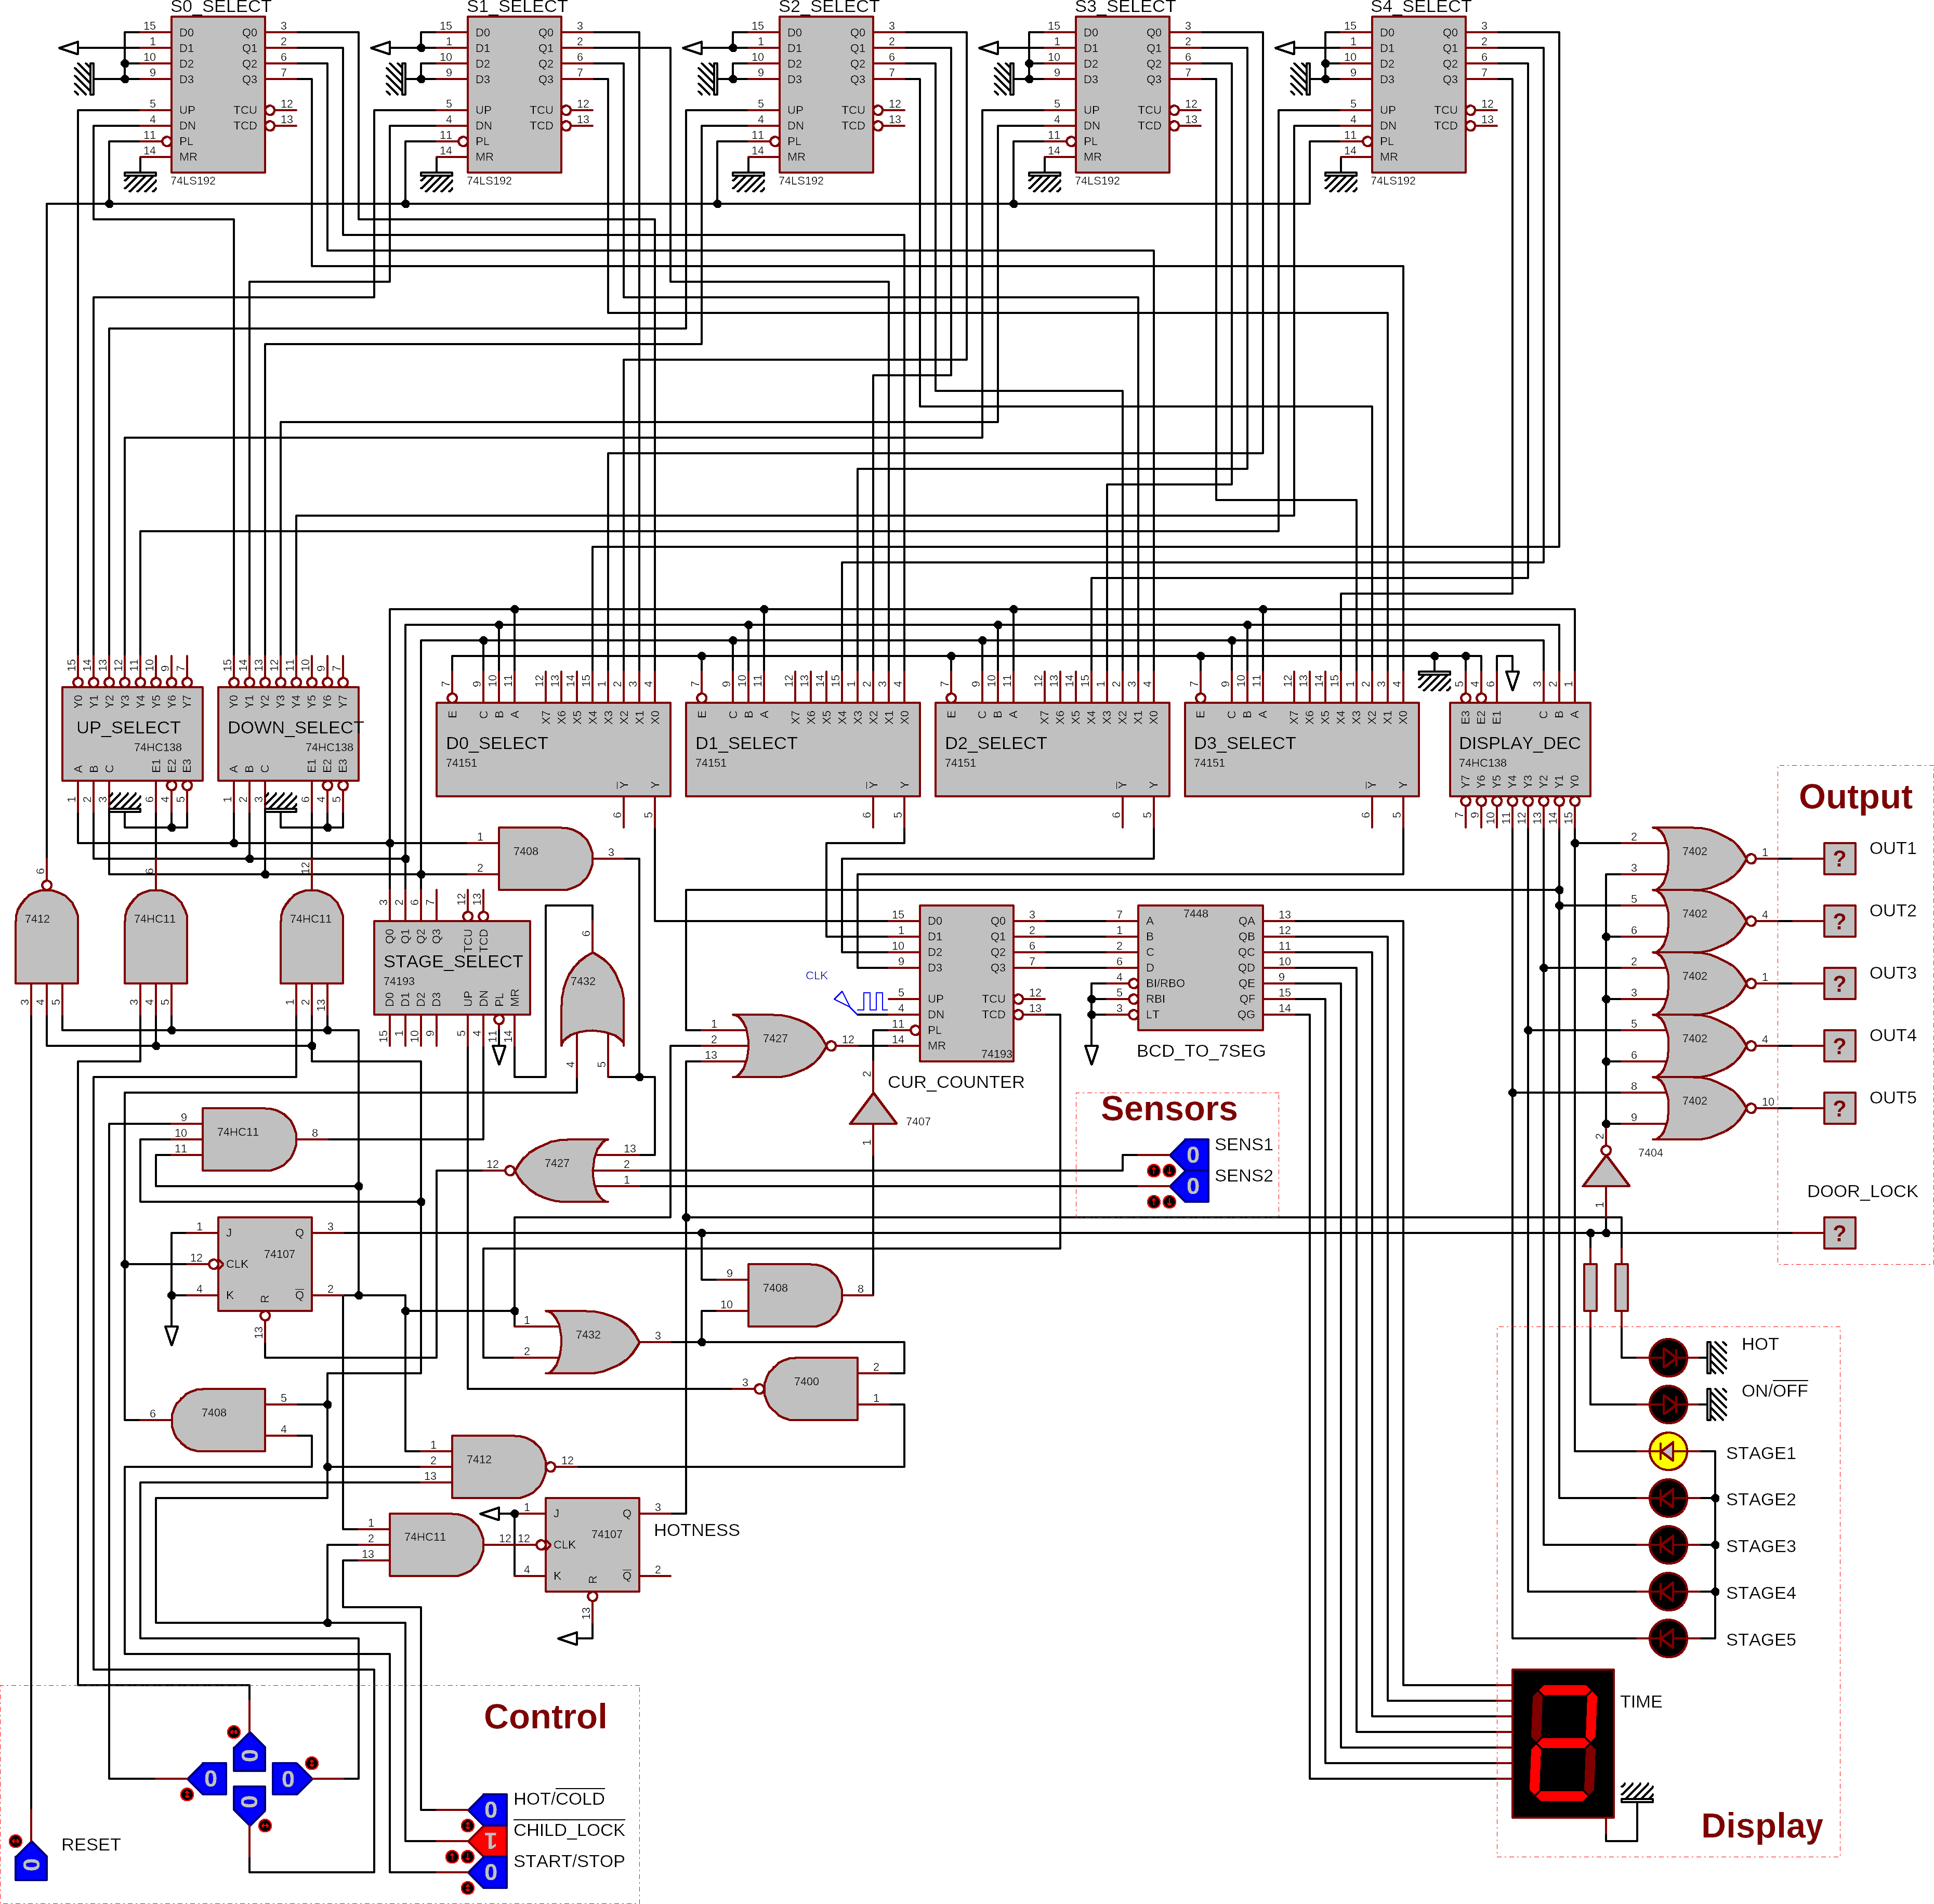
\includegraphics[width=\textwidth]{figs/schema.png}
	\caption{طرح پیشنهادی برای مدار}
	\label{fig:schema}
\end{figure}

در این مدار شمارند‌ه‌های
\LRE{\texttt{SX\_SELECT}}
زمان هر یک از ۵ فاز را مقداردهی می‌کنند.

تراشه‌های
\LRE{\texttt{XX\_SELECT}}
در زیر این شمارنده‌ها، برای انتخاب مسیر منتهی به شمارنده‌ی فعلی استفاده شده‌اند.یعنی با توجه به فاز فعلی عملیات، پایه‌ی های شمارنده‌ی مربوط به این فاز را به قسمت پایینی مدار متصل می‌کنند.
\LRE{\texttt{UP\_SELECT}}
و
\LRE{\texttt{DOWN\_SELECT}}
به پایه‌های
\LRE{\texttt{UP}}
و
\LRE{\texttt{DOWN}}
شمارنده متصل می‌شوند و
\LRE{\texttt{DX\_SELECT}}
ها به خروجی شمارنده متصل می‌شوند.
\LRE{display decoder}
خروجی مربوط به فاز فعلی عملیات را فعال می‌کند.
شمارنده‌ی
\LRE{stage select}
برای انتخاب فاز استفاده می‌شود. تراشه‌ی
\LRE{current counter}
وظیفه‌ی شمارش معکوس فاز فعلی عملیات را بر عهده دارد.

\section{پیوست‌ها}

\LRE{\attachfile[
author=احمدیان، رسولی، مظفری,
description=فایل شبیه‌سازی مدار پیشنهادی با فرمت
\LRE{DSN},
icon=Paperclip,
color=0.5 0.5 0.5,
print=false,
subject=فایل شبیه‌سازی مدار پیشنهادی با فرمت
\LRE{DSN},
zoom=false]{../simulation/6.dsn}}
فایل شبیه‌سازی مدار پیشنهادی با فرمت
\LRE{DSN}